\chapter{Contexte Entreprise}
\section{Entreprise d'accueil}
L’accueil téléphonique en France est principalement utilisé par les professions libérales 
mais également pour les entreprises de toutes tailles souhaitant avoir un accueil téléphonique.
Cette profession dispose de sa chambre professionnelle  le « SIST ». \newline

Le SIST regroupe 60 centres d’accueil partout en France cela représente 
8000 hôtesses d'accueil téléphonique et 150 millions d'appels entrant traités par an. 
Le principe de l’accueil téléphonique est de ne rater aucun appel téléphonique 
pour ne pas perdre de potentiel client. \newline

Le fait de confier sa ligne téléphonique à des professionnels 
permet d’avoir un accueil téléphonique de qualité.

Cela permet également de réduire drastiquement les coûts qu’aurait une entreprise à engager 
une ou plusieurs personnes à temps plein pour répondre aux appels.\newline

Créée en 1992 par ses actuels dirigeants, Eurice est spécialisée dans la gestion d'appels entrants.

Eurice est à la fois opérateur et fournisseur de solutions techniques de par ses services:\newline
\begin{itemize}
	\item L'accueil téléphonique fourni par un plateau de réception des appels 
	au sein des locaux de l'entreprise, qui peut aussi parfois servir d’environnement de pré-production 
	avant le déploiement de mise à jour chez les centres d'appels client.

	\item Le développement de solutions pour les centres d'appels: logiciel de gestion d'agenda, 
	répartiteur d'appel, portail client et applications mobiles, tous les logiciels utilisés à Eurice 
	et vendus au client, cela permet entre autre de connaître le besoin avec plus de précision 
	car nous sommes clients de nos propres produits. \newline
\end{itemize}
Chaque année, Eurice gère pour le compte de ses clients près 
d'un million d'appels décrochés en moins de 3 sonneries.
\newpage

\section{Organisation de l'entreprise}
\begin{figure}[h]
	\centering
	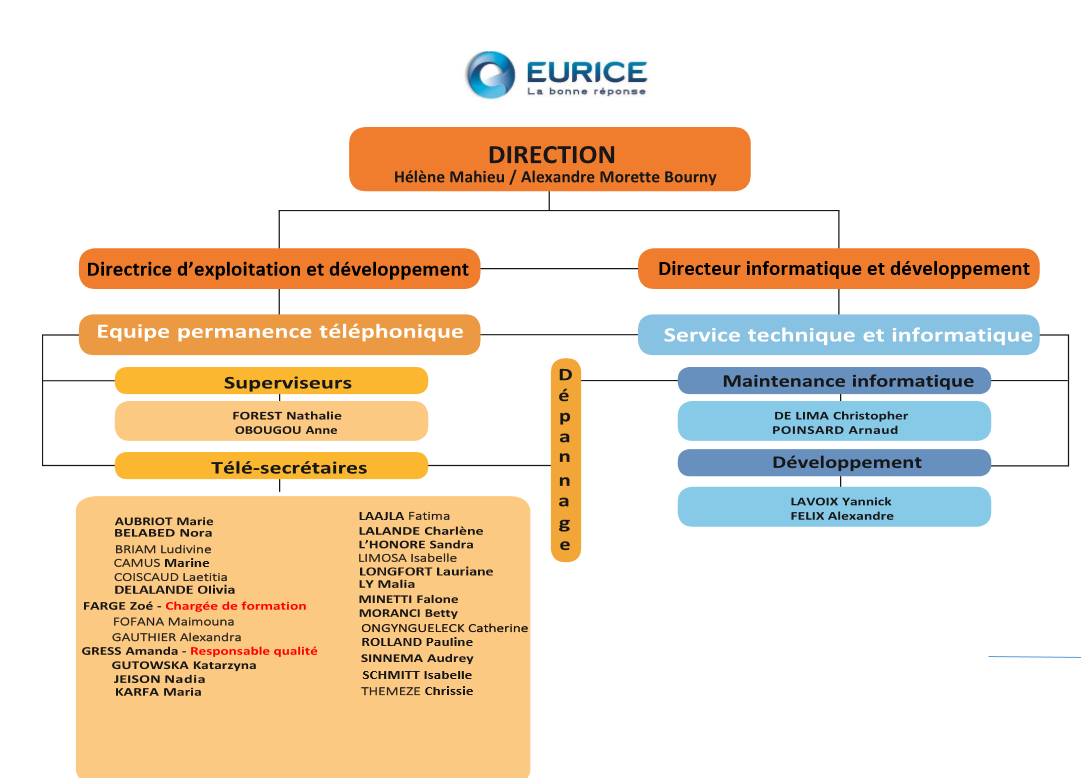
\includegraphics[width=0.8\linewidth]{Images/organigramme_fonctionnel}
	\caption{Organigramme Fonctionnel}
	\label{fig:organigrammefonctionnel}
\end{figure}

\section{Contexte Métier}
Il existe deux type de logiciels développés à Eurice: 
les logiciels utilisés pour la téléphonie dont le développement est réalisé par Mr. Morette-Bourny 
et les logiciels de gestion d'agenda qui sont réalisés par l'équipe de développement. \newline


\subsection{Callibri}
Il s'agit de l'application principale pour un centre d'appel. 
Ce logiciel permet la gestion de plusieurs dossiers avec leur agenda, 
avoir une communication entre la secrétaire et le client via les instructions et les messages. 
un système de scripting soutient l'opératrice lors du traitement d'un appel, 
c'est le support du pré-traitement et du post-traitement de l'appel. \newline

\gls{Callibri} s'interface avec le système d'appel pour automatiquement ouvrir le dossier correspondant 
au numéro appelé, cela permet de gagner un temps conséquent 
et de rendre transparent l'appel au yeux de l'appelant qui ne sait pas 
que son appel est décroché dans un centre d'appel. \newline


L'application utilise pour la majeure partie de l'interface des pages web grâce 
à la librairie Essentials Objects utilisant un moteur chrome embarqué.
Le reste de l'interface qui comprend le menu et la fenêtre native est réalisé en WPF. \newline

Les pages web utilisent le JavaScript avec jquery, 
le JavaScript s'interface avec le code CSharp de l'application qui contient tout le traitement, 
les accès à la base de données ainsi que la communication réseau. \newline

\gls{Callibri} étant utilisé sur plusieurs postes accédant à des ressources communes, 
le logiciel communique via messages UDP aux autres postes, pour, par exemple, éviter de prendre 
un rendez-vous sur le même créneau libre. \newline

\paragraph{Fonctionnalités \newline}
Les fonctionnalités principales de \gls{Callibri} sont divisés en plusieurs parties: \newline
\begin{itemize}
    %parler des fiches client en plus des dossiers
    \item Dossiers: \gls{Callibri} permet la création de dossier qui représente un client,
    il contient les coordonnées de ce dernier, les différents numéros de téléphone ainsi que les éléments
    de facturation et de l'agenda. \newline

    \item Gestion des instructions: ce sont les démarches 
    à suivre ou des informations laissées par le client aux opératrices, cela peut indiquer les habitudes du client, 
    des créneaux d'absence, informations d'accès ou autres. \newline 


    \item Scripting: le scripting permet de personnaliser le fonctionnement du dossier,
    cela peut être dans le traitement d'un appel ou d'un ajout de rendez-vous mais
    peut aller aussi jusqu'à l'affichage de fenêtres personnalisées lors d'un appel pour le dossier 
    \newline
    
    \item Messages: les messages sont le moyen de communication privilégié pour les opérateurs,
    ils permettent une communication direct au client.
    \newline

    %agenda/semaines type etc
    \item Gestion de l'agenda: c'est la partie centrale de \gls{Callibri} ou sont affichés les rendez-vous,
    les créneaux libres et les informations pertinentes pour les créneaux pris
    \newline
    
    \item Organigrammes d'entreprise: \gls{Callibri} a été prévu pour répondre 
    aux besoins de clients divers et variés. L'organigramme d'entreprise permet rapidement
     de visualiser la hiérarchie de l'entreprise, ses différents services ainsi 
     que chaque salarié attaché à ces services. \newline
\end{itemize}


%web 2
\subsection{Site client}
Le site client comme son nom l'indique est la partie accessible au client de l'agenda \gls{Callibri},
les fonctionnalités diffères légèrement par rapport à l'agenda de l'opérateur mais l'interface 
visuelle reste exactement la même, le site permet aussi de consulter les messages reçus et de les archiver, de même pour les instructions,
le client a aussi accès, s'il est client, à l'agenda web RDV Médicaux.\newline
\newpage



\section{Focus sur le service du stage}
Je fais partie de l'équipe développement qui est composé de Yannick Lavoix et de moi-même, 
notre objectif est d'ajouter des fonctionnalités aux logiciels existant, 
les maintenir et créer de nouvelles solutions comme c'est le cas avec ma mission.\newline

